\documentclass[12pt, oneside]{article}
\usepackage[letterpaper, margin=1in, headsep=0.5in]{geometry}
\usepackage[english]{babel}
\usepackage[utf8]{inputenc}
\usepackage{amsmath}
\usepackage{amsfonts}
\usepackage{amssymb}
\usepackage{tikz}
\usetikzlibrary{quotes, angles}
\usepackage{graphicx}
%\usepackage{pgfplots}
%\pgfplotsset{width=10cm,compat=1.9}
%\usepgfplotslibrary{statistics}
%\usepackage{pgfplotstable}
%\usepackage{tkz-fct}
%\usepackage{venndiagram}

\usepackage{fancyhdr}
\pagestyle{fancy}
\fancyhf{}
\rhead{\thepage \\Name: \hspace{1.5in}.\\}
\lhead{BECA / Dr. Huson / 10.3 Geometry\\* 25 October 2018}

\renewcommand{\headrulewidth}{0pt}

\begin{document}
\subsection*{Deltamath warmup}
Show your work. For graphs, use a pencil and straight edge.
  \begin{enumerate}

\subsubsection*{Graphing linear functions}

\item Two functions are shown in the table, $f(x)$ and $g(x)$.
\begin{enumerate}
  \item Plot the points on the graph. Draw and label straight lines for each function.
  \item Label the point $P$ where $f(x)=g(x)$. Add that row to the table.
  \item Circle the $y$-intercepts of each function in the table.
  \item Write the line differences next to the table to find the slopes.
  \item Write down the equations of both functions.
\end{enumerate}}

  \begin{center}
    \begin{tabular}{|c|r|r|}
    \hline
    $x$ & $f(x)$ & $g(x)$\\
    \hline
    0 & 2 & 0\\
    \hline
    2 & 3 & 1.5 \\
    \hline
    4 & 4 & 3\\
    \hline
    6 & 5 & 4.5\\
    \hline
    &  & \\
    \hline
    \end{tabular}
  \end{center}
%Graph the function as a line over the domain $-1 \leq x \leq 3$.

  \begin{center} %4 quadrant regents grid w T-Chart
  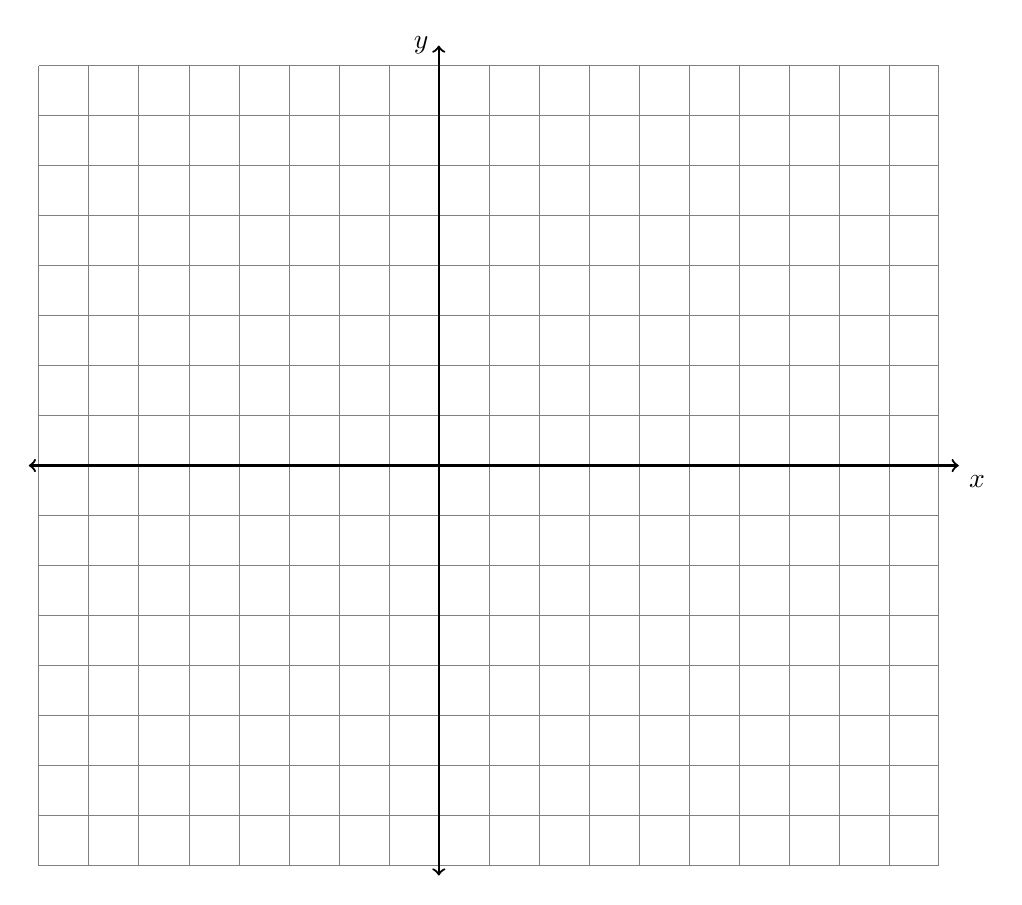
\begin{tikzpicture}[scale=.635]
    \draw [help lines] (-8,-8) grid (10,8);
    \draw [thick, <->] (-8.2,0) -- (10.4,0) node [below right] {$x$};
    \draw [thick, <->] (0,-8.2)--(0,8.4) node [left] {$y$};
  \end{tikzpicture}
  \end{center}

\end{enumerate}
\end{document}
